
\section{Experiments}\label{sec:exp}
To evaluate the effectiveness of our approach, we conduct a series of comparison experiments and ablation studies on two widely used datasets,~\emph{i.e.,} YouTubeVOS \cite{xu2018Youtube} and DAVIS \cite{davis_2017}, under different settings.
%We test on two datasets, YouTubeVOS \cite{xu2018youtube} and DAVIS \cite{davis_2017}, to compare the proposed STSENet with state-of-the-art methods. %Several ablation studies are conducted to prove the effectiveness of spatial details and temporal information in video inpainting.

\subsection{Experimental Settings}
\noindent \textbf{Mask Setting.} Considering different real-world applications, we test four kinds of mask settings in this paper, which are different in shapes and positions of the missing regions. 
%The first and the second settings aims to recover rectangular regions, which are common in watermark removal.
\begin{enumerate}
\item Fixed square mask: The size and position of the missing square regions are fixed through the whole video. 
\item Moving square mask: The position and size of the square masks change over frames. 
\item Free-from mask: We apply irregular masks which imitate hand-drawn masks on each frame, following \cite{liu2018partialinpainting}. 
\item Foreground object mask: This type of mask is defined to line out foreground objects in videos and used for testing object removal.
\end{enumerate}

\noindent\textbf{Dataset.} 
YouTubeVOS and DAVIS are widely used for evaluating video inpainting results in recent studies.
YouTubeVOS consists of 4,453 video clips that contain more than 70 categories of common objects. 
The videos are split into three parts, 3,471 for training, 474 for validation, and 508 for testing. Since YoutubeVOS has no dense foreground mask annotations, we only use it for evaluation under mask settings (1), (2), and (3). 
% 
DAVIS dataset contains 90 video sequences that are annotated with foreground object masks for test and 60 unlabeled videos for training.


\begin{figure*}[tb]
	\centering
	\includegraphics[width=\textwidth]{viszong} % Reduce the figure size so that it is slightly narrower than the column. Don't use precise values for figure width.This setup will avoid overfull boxes. 
	\caption{Comparison with state-of-the-art methods on the YouTubeVOS dataset under different mask settings. Our method produces results with more complete object structures and finer details. %\cxj{Modify reference number at last.} 
	}
	\label{viszong}
\end{figure*}



\begin{table*}[t]
	\caption{Comparisons with four state-of-the-art methods on YouTubeVOS. Our method outperforms all other methods on three metrics, with fast inference speed.}\smallskip
	
	\centering
	\resizebox{2.0\columnwidth}{!}{
		\smallskip\begin{tabular}{c|c|c|c|c|c|c|c|c|c|c }
			\hline
			&\multicolumn{3}{c|}{Fixed Square Mask}& \multicolumn{3}{c|}{Moving Square Mask}&\multicolumn{3}{c|}{Free-Form Mask}&Inference \\
			\cline{2-10} 
			&PSNR & SSIM & FID & PSNR & SSIM & FID & PSNR & SSIM & FID&Speed (fps)\\
			\hline
			Edge-Connect \cite{nazeri2019edgeconnect} &28.6446 &0.9484  &   38.2116  &    
			30.7478 & 0.9647 &  16.2739  &
			25.6693  & 0.9088 &  43.0366&22.81 \\
			\hline
			CombCN \cite{wang2019video} &27.9668 & 0.9515 &  40.7199  &     
			31.5776    & 0.9678 &  13.8383&   
			32.1862 & 0.9626 & 19.1191 &8.1634 \\
			\hline
			
			
			DVI \cite{Kim_2019_CVPR1}& 28.0846&0.9468 &  39.9377  & 
			36.8598    & 0.9728 &7.2315  &
			33.5549    & 0.9646 & 9.3797&1.2275  \\
			\hline
			DFVI \cite{Xu_2019_CVPR} &29.0531 & 0.9497 &  32.8860  & 
			37.8241& 0.9772 &6.3746  &
			32.6287 &0.9618  &  11.1501&0.5620 \\
			\hline
			
			\hline
			
			
			
			Ours &\textbf{30.0590} &\textbf{0.9543}&   \textbf{27.2431} &
			\textbf{38.8186} & \textbf{0.9824} & \textbf{2.3455} &
			\textbf{35.9613}  & \textbf{0.9721}&  \textbf{ 5.8694} &5.1546\\
			
			\hline
			
			
		\end{tabular}
	}
	\label{tab:sem}
\end{table*}





\noindent \textbf{Implementation details and Evaluation Metrics.} 
All the models are tested on a TITAN X (Pascal) GPU with frame size $256 \times 256$.
For training data, we randomly sample a training clip every 40 frames from each video in the dataset. Our training process consists of three steps. First, we train ENet with learning rate set as $1e-4$ for $G^E$ and $1e-5$ for $D^E$. 
Then we train TexNet while fixing ENet. The learning rate is set as $1e-4$ for $G^T$, and $4e-4$ for $D^T$.
We first train ENet and TexNet without flow-constrained losses, and then add the flow losses to finetune the networks.
%ensemble module is finally trained while fixing all the other modules. Learning rate is $1e-4$.
An Adam optimizer with $\beta=(0.9, 0.999)$ is used for all sub-network training.
%We do not use weight decay.
As for the hyper-parameters, we set $\lambda_1=10.0,\lambda_2=0.2$.
%, \lambda_3=0.1$.

Different data preparations and evaluation metrics are used according to mask settings. We randomly generate masks for training videos in terms of mask settings (1), (2), and (3). 
Masked videos are used for testing.
Three commonly-used metrics, including structural similarity index (SSIM) \cite{wang2004image}, peak signal-to-noise ratio (PSNR), and Fr{\'e}chet Inception Distance (FID) \cite{heusel2017gans} are used to quantitatively evaluate the performance of our method. 
For the mask setting (4), for each training video, we randomly select a test video from the 90 test videos in the DAVIS dataset and apply its masks for the current training video with random rotation, scaling, and translation.
Our inpainting network is first trained on the YoutubeVOS dataset and then finetuned on the DAVIS dataset. 
Since there are no ground truth videos available for this mask setting, we can not conduct quantitative evaluations to measure the output quality. In contrast, a user study is conducted for video foreground object removal.  


 


\subsection{Evaluation of Video Inpainting on YouTubeVOS}
We compare the proposed method with four state-of-the-art video inpainting methods \cite{nazeri2019edgeconnect,wang2019video,Kim_2019_CVPR1,Xu_2019_CVPR}
for the first three mask settings on the YouTubeVOS dataset.
%
We train \cite{nazeri2019edgeconnect,Xu_2019_CVPR} using their published codes and re-implement \cite{wang2019video} according to their paper. As for \cite{Kim_2019_CVPR1}, we use the officially provided model.

The quantitative results and inference speeds are reported in Table~\ref{tab:sem}.
It shows that our method outperforms state-of-the-art methods on the three metrics, demonstrating the effectiveness of introducing structure guidance into video inpainting.
Moreover, our method is also very efficient, e.g., four times faster than DVI \cite{Kim_2019_CVPR1} and nine times faster than DFVI \cite{Xu_2019_CVPR}. 
%We also notice that the best performance is typically obtained when using moving square masks for each individual approach. It indicates that these inpainting network can learn complementary information from neighboring frames.
Some inpainting examples are shown in Fig.~\ref{viszong}.
Compared with existing methods, the inpainting results predicted by our method are more realistic with finer details. 
We can observe that the frames completed using our method contain sharper object boundaries. This is achieved by the effectiveness of structure information in video inpainting.
%
It can also be seen that our method produces temporally smooth results when observing neighboring frames. 
%\cxj{show results?}


Compared with the 2D image inpainting method Edge-Connect\cite{nazeri2019edgeconnect},
which also predicts edges to represent the target structure,
our method greatly increases the completion performance by leveraging neighboring frames to complete edges and synthesize textures. 
Thus, our method can generate more temporally coherent and realistic contents. The inference speed of Edge-Connect is faster than our method since it does not consider axillary temporal information between frames. 
%
Compared with the second-best video inpainting method DFVI \cite{Xu_2019_CVPR}, our method produces frames with finer structural details. Besides, only ENet and TexNet are used to directly predict final outputs in the testing period in our method, while DFVI requires iterative pixel propagation. Thus the inference speed of our method is much faster than that of DFVI.
%
%% Time performance analysis 
Both the quantitative and qualitative results demonstrate that our method is not a naive extension to utilize structure information in video inpainting.
The well designed network architecture fully exploits structural guidance in video inpainting and brings large performance gain.




\begin{figure}[!t]
	\centering
	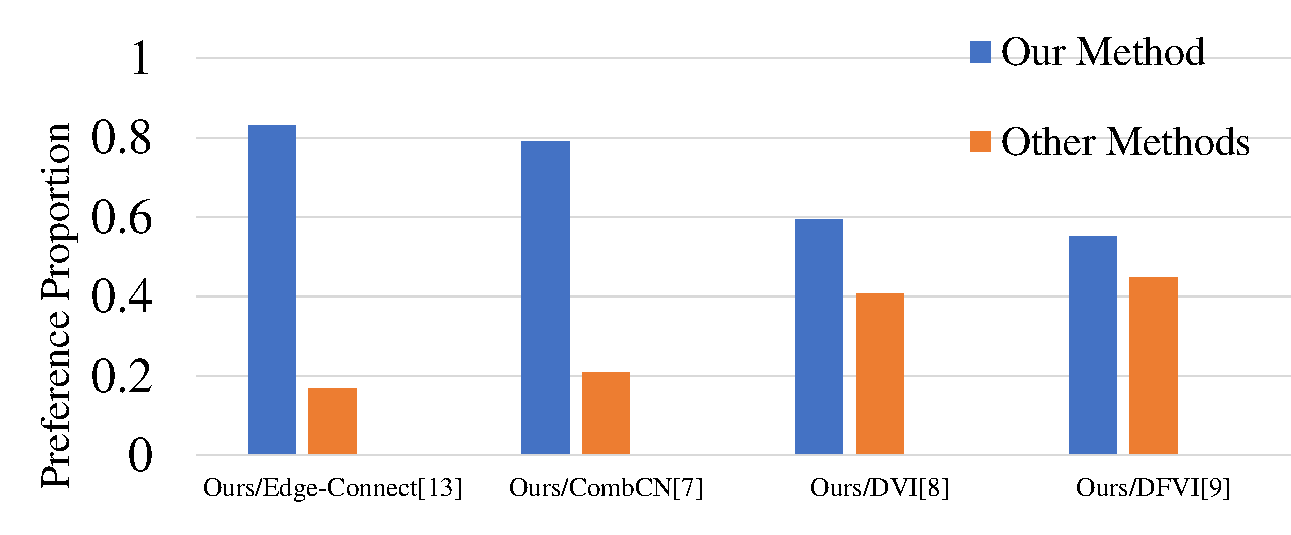
\includegraphics[width=1.0\columnwidth]{userstudy} % Reduce the figure size so that it is slightly narrower than the column. Don't use precise values for figure width.This setup will avoid overfull boxes. 
	\caption{Results of user study. The restored videos using our method are preferred by more participants compared with other state-of-the-art methods. }
	\label{userstudy}
\end{figure}



\begin{figure}[!t]
	\centering
	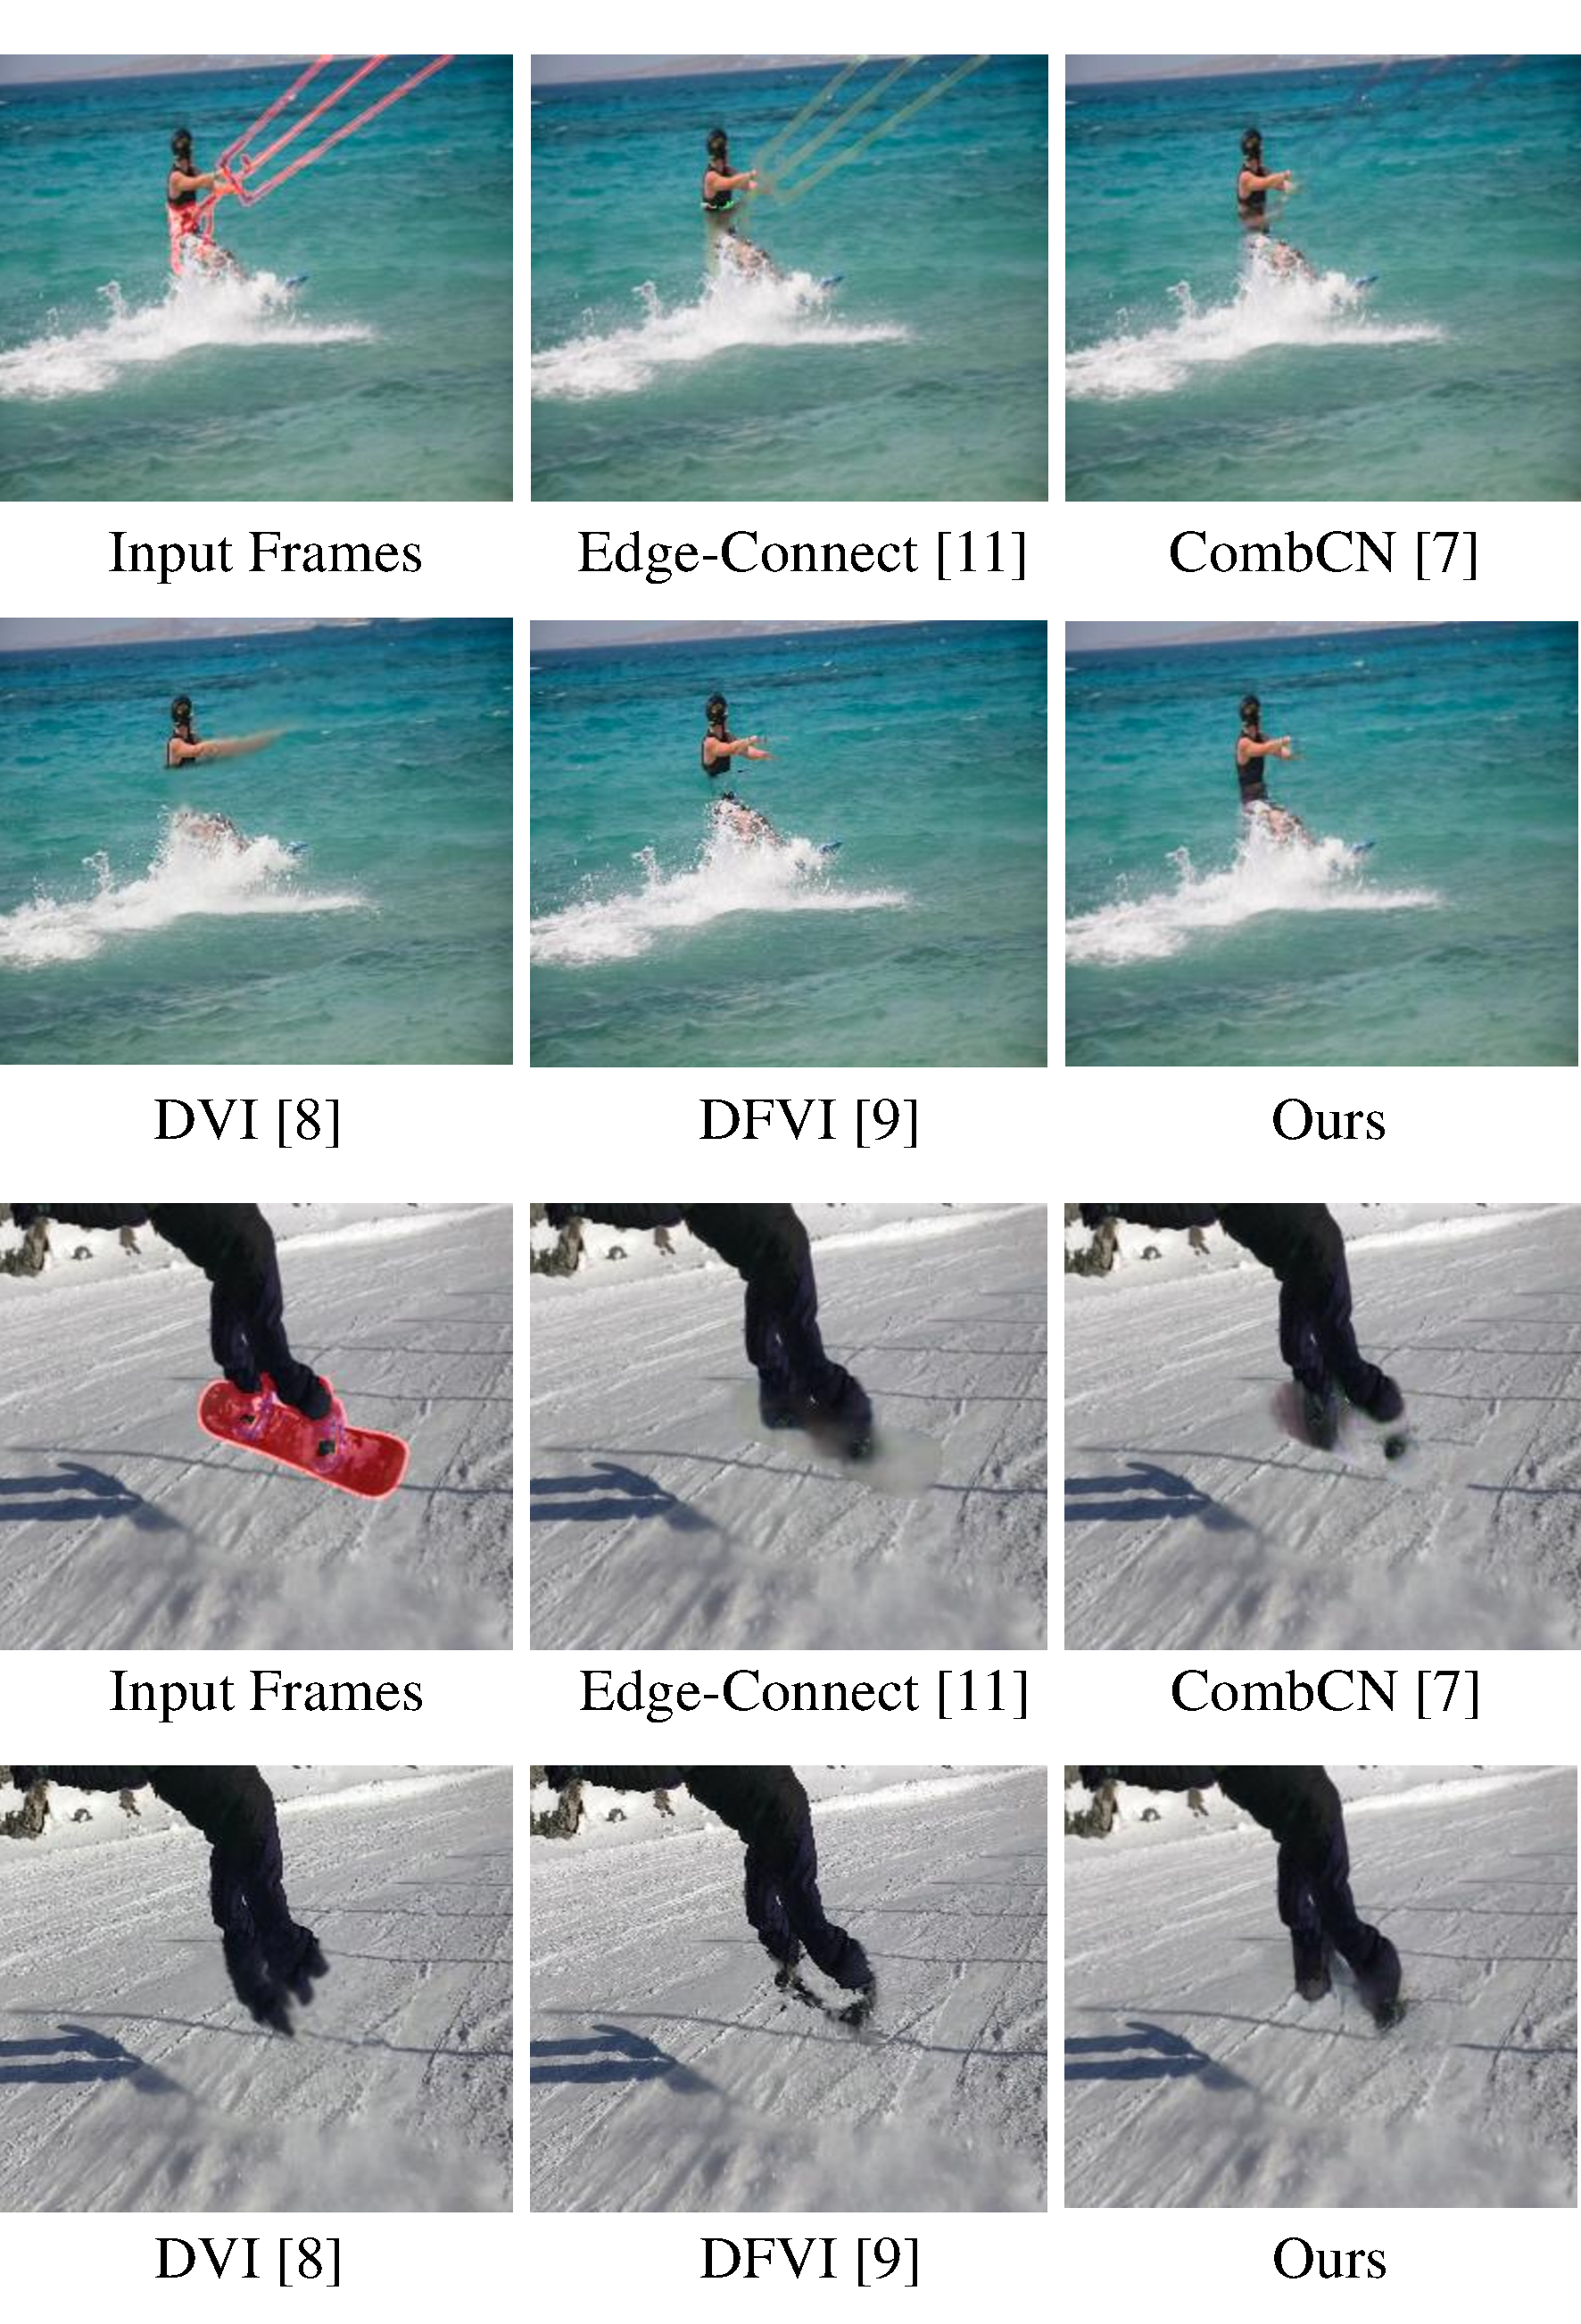
\includegraphics[width=0.85\columnwidth]{vis_forg} % Reduce the figure size so that it is slightly narrower than the column. Don't use precise values for figure width. This setup will avoid overfull boxes. 
	\caption{Results of object foreground removal. The red masks in input frames indicate the objects to be removed. Our method produces results with plausible structures and details.}
	\label{vis_forg}
\end{figure}


\subsection{Object Removal on DAVIS}


In regard to the foreground object mask setting that aims to remove undesired objects in videos, there is no ground truth for quantitative evaluation. 
Therefore, we conduct a user study on the DAVIS dataset to evaluate the visual quality of our method, compared with the four methods \cite{nazeri2019edgeconnect,wang2019video,Kim_2019_CVPR1,Xu_2019_CVPR}.
%
In each test, we show three videos to the subject at the same time. The original video with red masks indicating objects to remove is shown in the middle, while the inpainting results of our method and one of the other four methods are shown on the two sides in random order.
%  
The subjects can watch the videos repeatedly to better evaluate the differences.
For each video triplet, the subject is asked to choose which inpainting video is preferred.
44 subjects participated in our user study. 
Each participant watched averagely 20 triplets. 
Therefore, each pair of methods is compared about 220 times.
%Each method is compared about 200 times.

%


\begin{table*}[!t]
	\caption{Ablation studies on YouTubeVOS. Structure inference, structure attention model, and flow constrained loss are demonstrated effective in video inpainting.}\smallskip
	
	\centering
	\resizebox{1.8\columnwidth}{!}{
		\smallskip\begin{tabular}{c|c|c|c|c|c|c|c|c|c|c }
			\hline
			&\multicolumn{3}{c|}{Fixed Square Mask}& \multicolumn{3}{c|}{Moving Square Mask}&\multicolumn{3}{c|}{Free-Form Mask}&Inference \\
			\cline{2-10} 
			&PSNR & SSIM & FID & PSNR & SSIM & FID & PSNR & SSIM & FID&Speed (fps)\\
			
			\hline
			
			
			TexNet &28.0174 &0.9494  &  42.7164   &    
			33.8131 &  0.9705  &8.2390    & 
			30.0680& 0.9390 & 20.6358&7.6335
			\\
			\hline
			+Edge  &29.5242 &  0.9520& 36.2097   &    
			37.6630    & 0.9798 &3.5161    &    
			33.8206    &0.9659  &    6.6651& 5.2356 \\
			\hline
			
			+SAM &29.9918 &  0.9533 &  27.4198  &    
			38.2433    & 0.9807 &   2.5083  &    
			35.7783    &0.9712  &   5.8786 & 5.1546\\
			\hline
			
			
			
			
			+Flow &\textbf{30.0590} &\textbf{0.9543}&   \textbf{27.2431} &
			\textbf{38.8186} & \textbf{0.9824} & \textbf{2.3455} &
			\textbf{35.9613}  & \textbf{0.9721}&  \textbf{ 5.8694} &5.1546\\
			
			\hline
			
			
		\end{tabular}
	}
	\label{tab:abl}
\end{table*}

The preference results in the user study are shown in Fig.~\ref{userstudy}. 
Comparing to Edge-Connect \cite{nazeri2019edgeconnect}, CombCN \cite{wang2019video}, DVI \cite{Kim_2019_CVPR1}, our results are preferred by a significantly larger portion of subjects.
%
When comparing with the flow-guided method DFVI~\cite{Xu_2019_CVPR}, our method is preferred by $55.24\%$ of the tests. 
Notably, our method is much faster than DFVI.
%
Fig.~\ref{vis_forg} shows two examples of object removal using different methods. 
We can see that the inpainted results generated by our methods are visually better than existing methods.
Compared to the blurry contents in the results of Edge-Connect, CombCN, and DVI, our method produces sharp object boundaries and fine visual details. Notably, though the completed contents using DFVI have sharp edges, the global structure of the human bodies is corrupted. In comparison, our method achieves more intact and plausible structure with fine details.
The results demonstrate the importance of utilizing structure information in video inpainting. 










\subsection{Ablation Study}
To demonstrate the effectiveness of each component in our network, we conduct a series of ablation studies on the YouTubeVOS dataset with the first three mask settings. 
%
We test four variants of our model. 
The baseline model `TexNet' only consists of the coarse-to-fine texture inpainting network without using edge maps as input and no SAM in the refinement module.
This model simply integrates neighboring frames to predict the missing content for the current frame.
%
Then we add the edge inpainting network ENet and feed the texture inpainting network with the completed edge maps to get the second model `+Edge'.
The third model `+SAM' is constructed by adding the structure attention module on the second model. 
Finally, we add the flow constrained loss during training to get our full model `+Flow'. Especially, we only add the flow constraints in the training stage, which means it brings no computation costs to the inference process.
The quantitative results are reported as in Table~\ref{tab:abl}. 

%

\subsubsection{Effect of Structure Clues}


\begin{figure}[t]
	\centering
	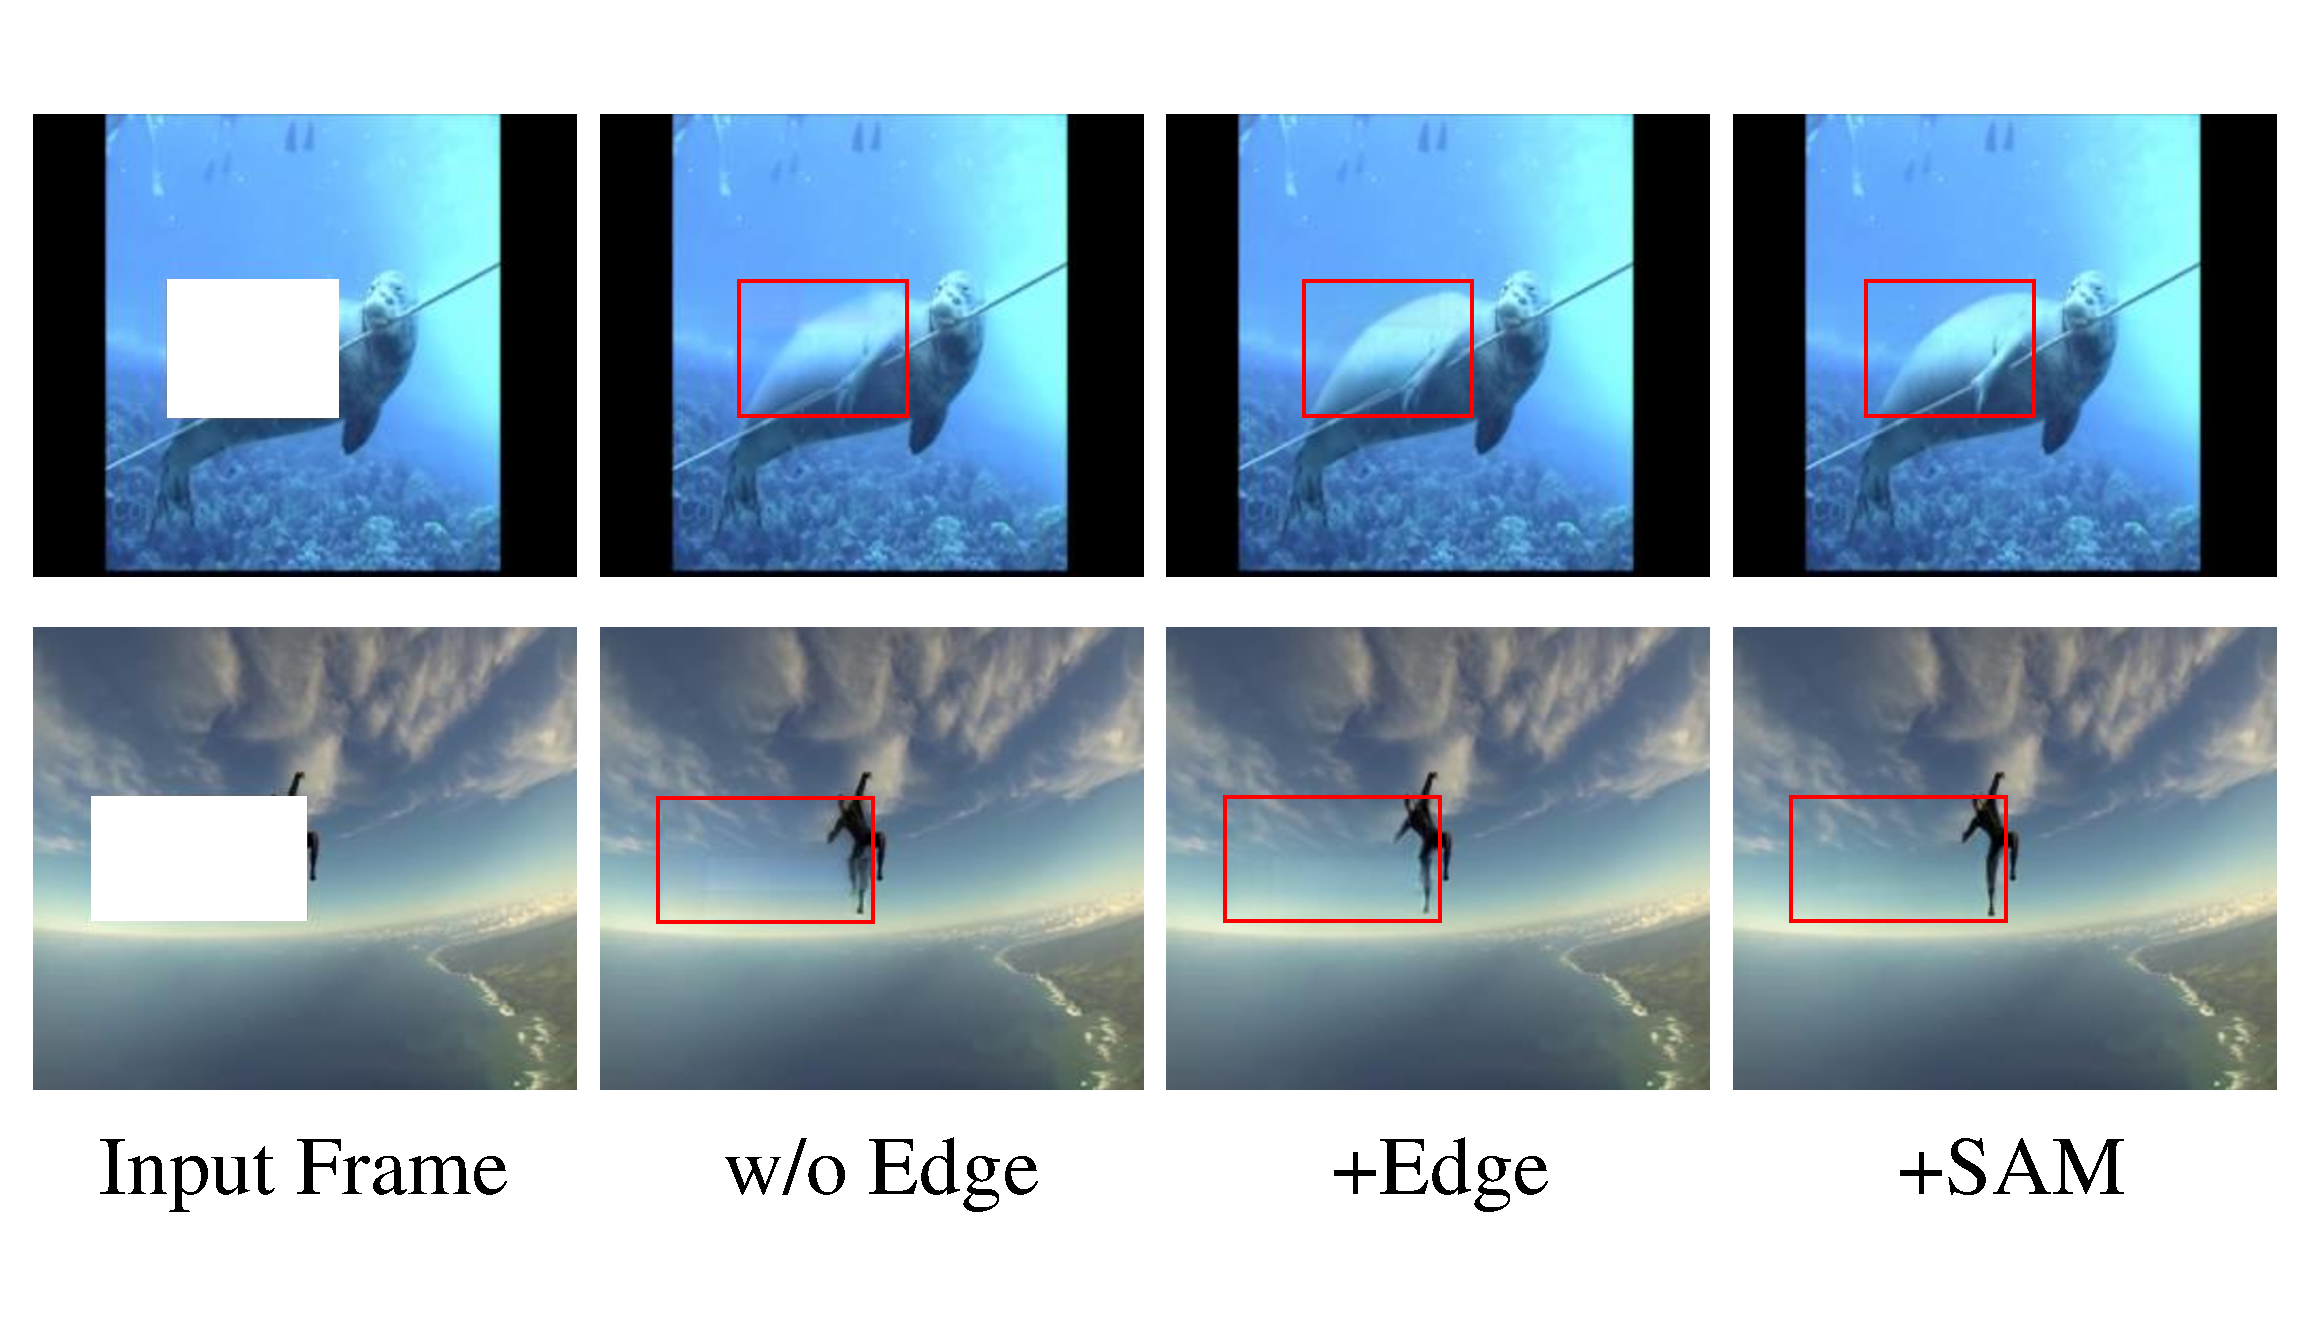
\includegraphics[width=0.97\columnwidth]{edgevis} % Reduce the figure size so that it is slightly narrower than the column. Don't use precise values for figure width.This setup will avoid overfull boxes. 
	\caption{Effects of structural guidance. By hallucinating edge maps first and then filling texture, we generate more completed and plausible target structure. Clearer boundaries can be obtained using the structure attention module.}
	\label{edgevis}
\end{figure}



In Table~\ref{tab:abl}, The model `+Edge' brings large improvement over the baseline model.
It indicates that sparse edges can provide effective structural guidance in video inpainting.
When we further add SAM, extra improvement is obtained, demonstrating that the spatial correlation between edges and textures can be better embedded and absorbed by the texture inpainting network than simply feeding the hallucinated edge maps as extra channels into TexNet.
The above analysis proves that the edge clues are effective guidance in video inpainting, which helps the network to predict more plausible frames with completed and detailed structure.
Indeed, the structure inference module ENet brings extra time cost to the baseline TexNet from 7.6335 \emph{fps} to 5.2356 \emph{fps}.
This is deserved because the inpainting quality is significantly improved.

Fig.~\ref{edgevis} shows the results generated using the three variants. 
It is obvious that after introducing structural guidance, the inpainted frames become more visually pleasing with sharper object boundaries. 
Besides, the edge maps predicted by our method are reasonable and clear, which well represent the image structure and show the strong edge inpainting ability of ENet. 
Thus, it is crucial to explore structural details in video inpainting.
 



%\begin{figure}[t]	
%    \centering
%    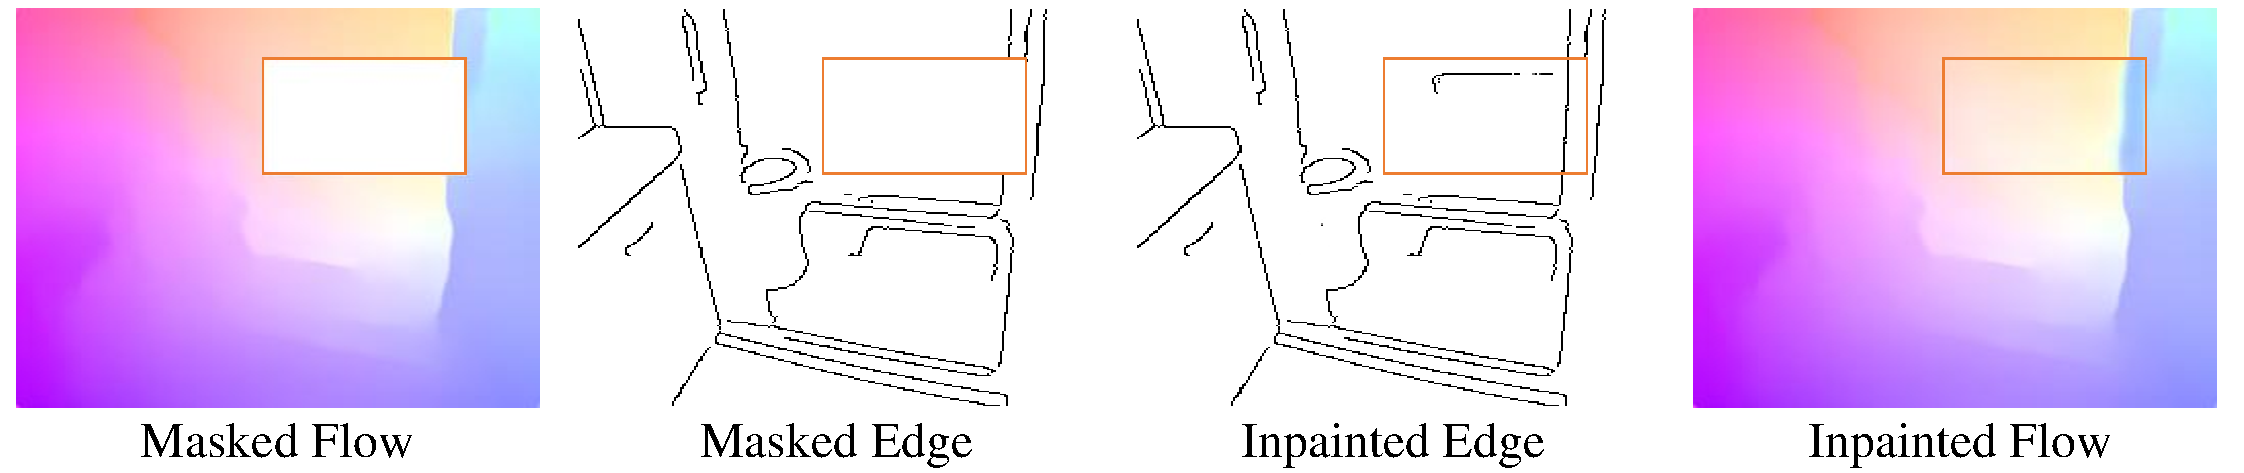
\includegraphics[width=1.0\columnwidth]{flowvis} % Reduce the figure size so that it is slightly narrower than the column. Don't use precise values for figure width.This setup will avoid overfull boxes. 
%    \caption{Visualized optical flow predicted by our method.}
%    \label{flowvis}
%\end{figure}


\begin{table}[t]
	\caption{Comparison of proposed structure attention module (SAM) and simple 2-layer spatial attention on YouTubeVOS. SAM is capable of the revealing potential correlation between structure information and video contents. }\smallskip
	\scriptsize
	\centering
	{
		\smallskip\begin{tabular}{c|c|c|c}
			\hline
			&\multicolumn{3}{c}{Free-Form Mask} \\
			\cline{2-4} 
			& PSNR & SSIM & FID\\
			
			\hline
			+Edge  &33.8206    &0.9659  &    6.6651 \\
			\hline
			
			+SimATT &34.4321    &0.9685  &   6.3125 \\
			
			\hline
			
			+SAM &\textbf{35.7783}    &\textbf{0.9712}  &   \textbf{5.8786}\\
			\hline
			
			
			
			
		\end{tabular}
	}
	\label{tab:sam_com}
\end{table}



\subsubsection{Comparison of Proposed Structure Attention Module and Simple Attention}

We propose a novel structure attention module (SAM) in TexNet to facilitate exploiting structure information of edge maps more effectively. This module is specifically designed for structural distilling in video inpainting. 
We conduct a comparison experiment between the proposed SAM and the commonly used simple 2-layer attention (SimATT) \cite{min2019two},~\emph{i.e.,} using a 2-layer convolution network to extract a spatial attention map from predicted edge maps, which is then applied to the same video feature as SAM. 
The model `+Edge' is used as the baseline.
%Compared with the SimATT, the proposed SAM considers the correlation between the edges and texture to generate the attention.
Results are shown in Table~\ref{tab:sam_com}.
The performance of SAM is better than that of SimATT. It is because that the proposed SAM is more effective in revealing potential correlation between structure information in edge maps and video contents. %Thus it is easier for TexNet to utilize structure information to obtain better results.




\begin{figure}[t]
	\centering
	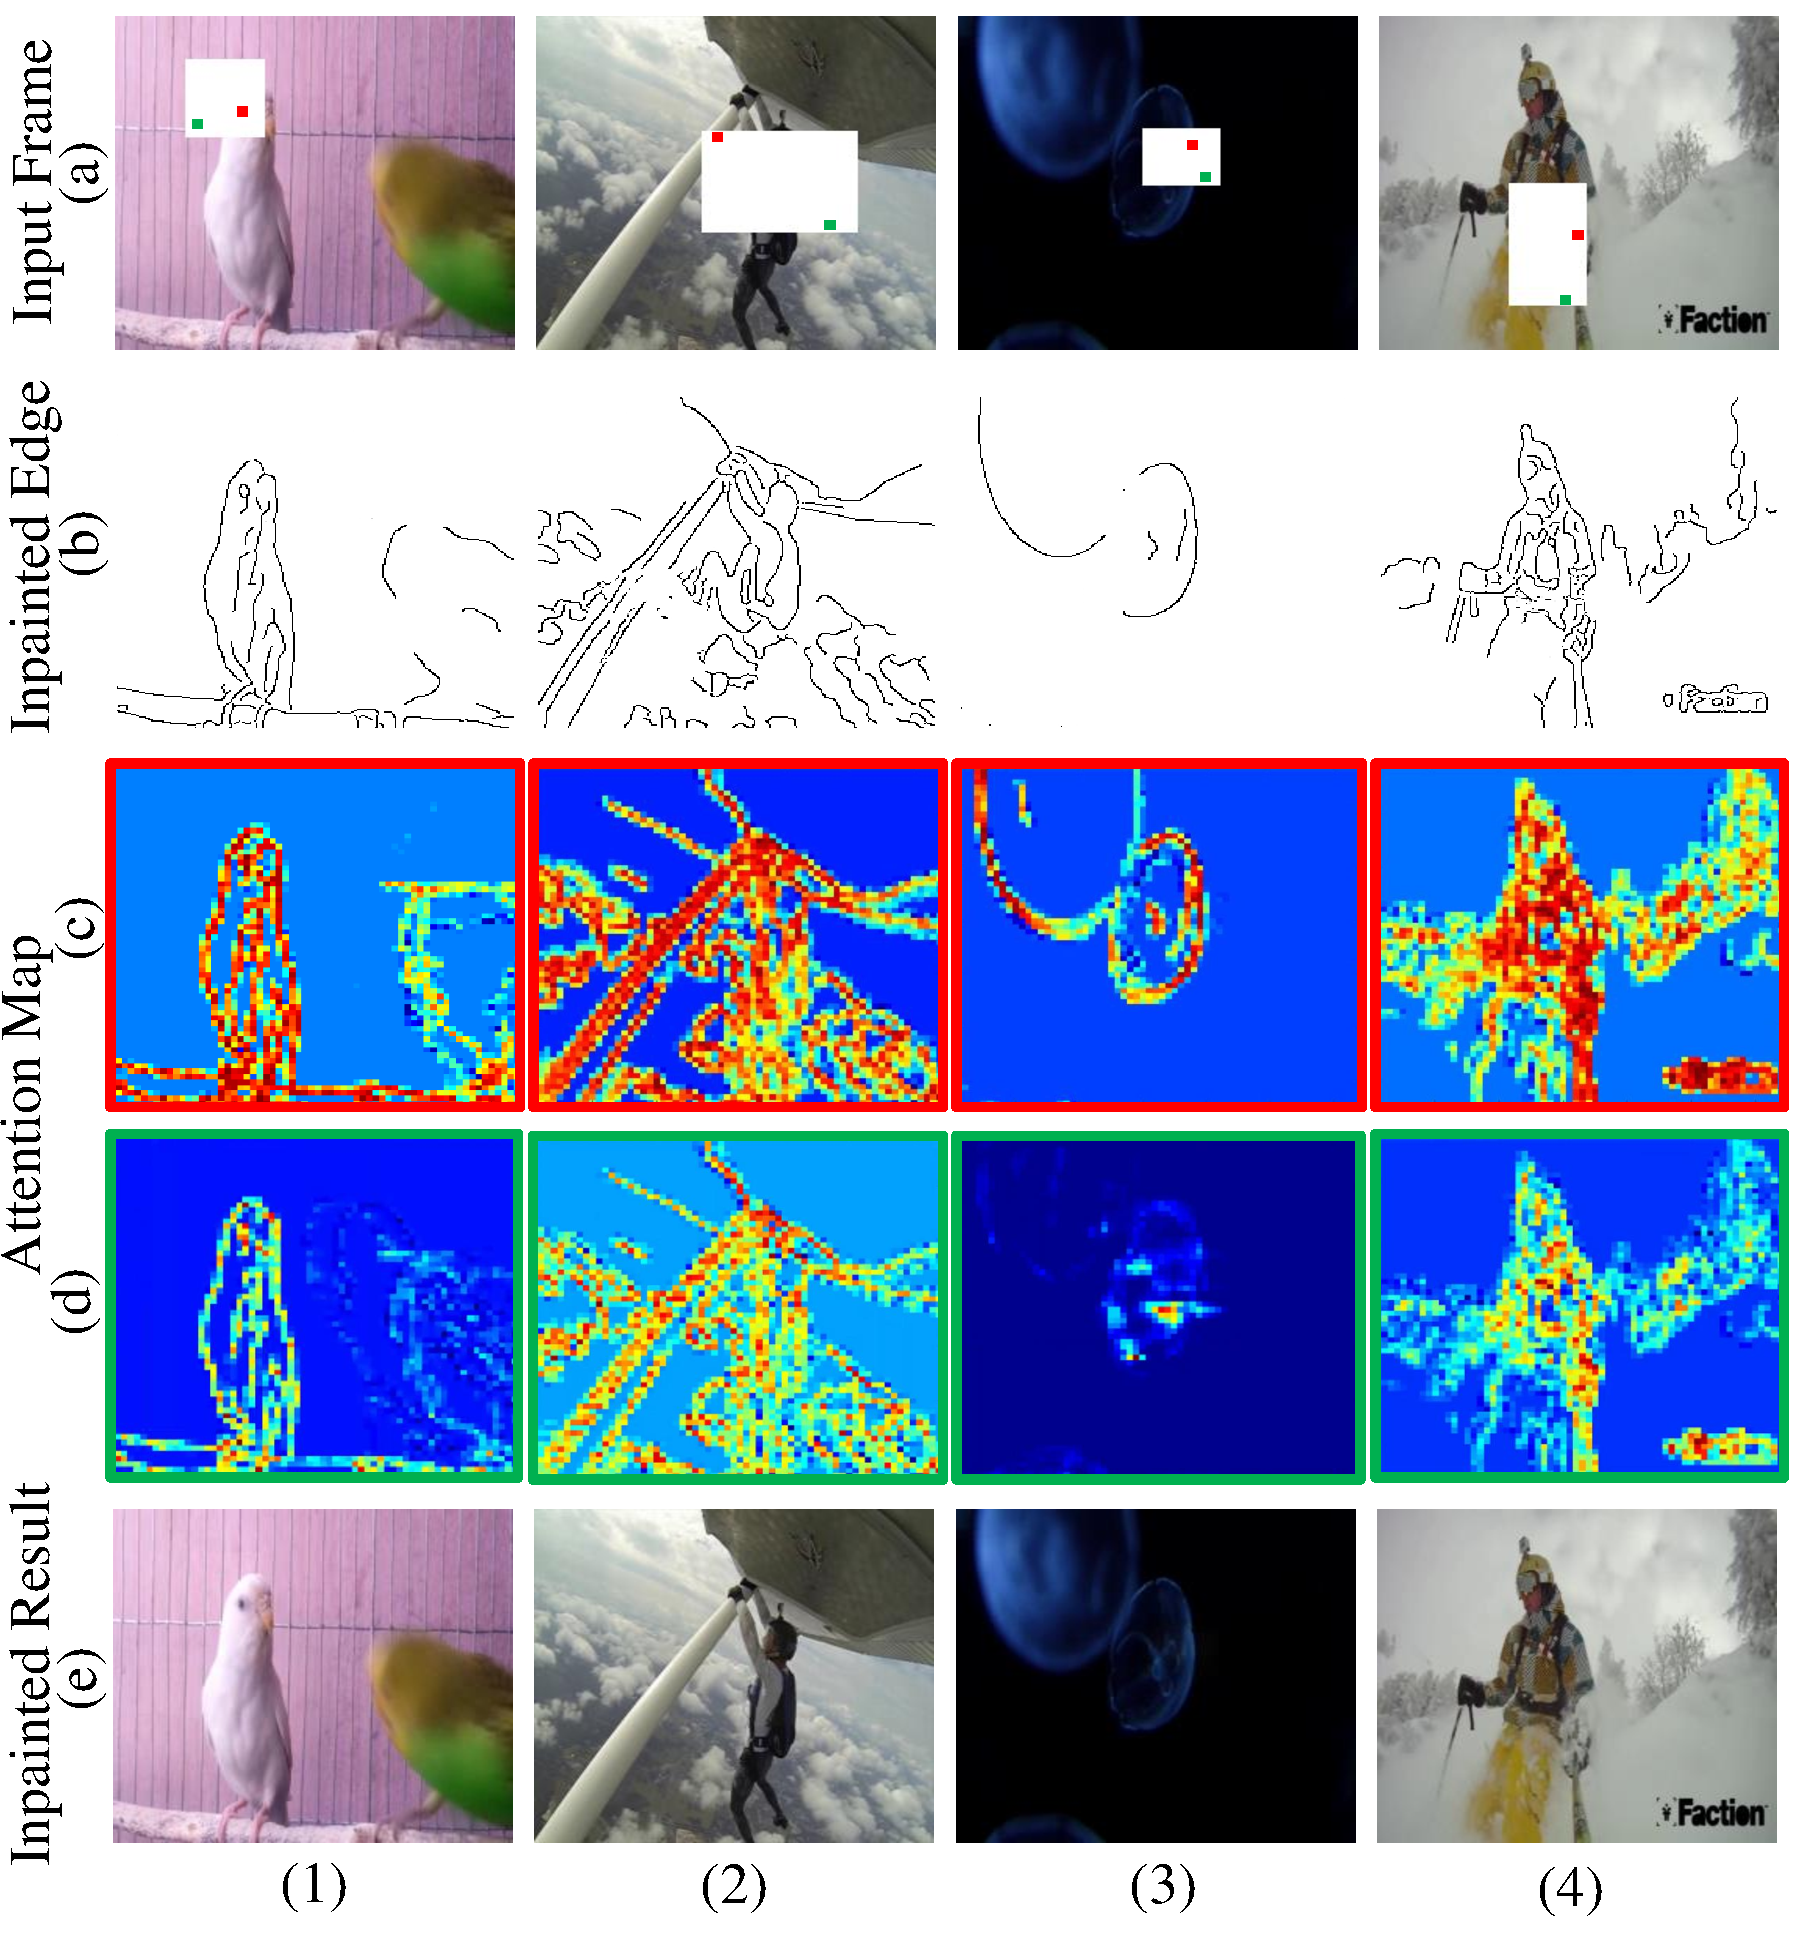
\includegraphics[width=1.0\columnwidth]{att} % Reduce the figure size so that it is slightly narrower than the column. Don't use precise values for figure width.This setup will avoid overfull boxes. 
	\caption{Visualization of the normalized attention map in proposed structure attention module. The attention map demonstrates the correlation between the selected pixel, which is denoted by red point on input frame, and all pixels on the whole input features.}
	\label{fig:att}
\end{figure}





\subsubsection{Visualization of Proposed Structure Attention Module}

To further reveal the effects of structure attention module in our framework, some visualization results are given in Fig.~\ref{fig:att}.
The red point in the input frame indicates the selected pixel to be inpainted, and the heat regions in the attention map are pixels related to that pixel.
It can be seen that, under the guidance of the edge structure, the inpainted pixel focuses on the texture around the object contours.
Thus, the generated texture in the missing regions will preserve a consistent contour according to the whole object shape, which makes the results visually reasonable.
Furthermore, the edge guidance also prevents the module from being disturbed by the background information, thus most of the heat regions are from the target and related objects.
In summary, the above observations prove that it is reasonable to introduce the edge guidance into frame inpainting, and the proposed structure attention module is an effective module in embedding the edge structure into the texture generation.








\subsubsection{Effect of Flow for Temporal Coherence}

%Temporal coherence is an important factor in video inpainting. 
We utilize temporal information to smoothen artificial flickers via two developed flow-guided warping losses during training. 
Table~\ref{tab:abl} shows that the quantitative performance is improved on all three mask settings by adding the flow guidance. Especially, we only add flow guidance in the training phase. 
Thus it brings performance gains without extra computation costs during testing.
%However, the performance improvement brought by the flow constraints is smaller than the gain caused by structural guidance.The reason is that the flow is only used in the training stage as temporal guidance, while the edge is used during the inference.
%It should be noted that predicting the completed optical flow among several frames takes more time than the edges during inference.
%Thus, we use the flow in training and the structure edge in both training and testing, which can achieve a good balance between the quality improvement and the inference efficiency. 
%
As Fig.~\ref{flow_vis} show, the synthesized contents in neighboring frames become more temporally consistent by adding the flow constrained losses.
This proves that the proposed two flow-guided constraints in edge and texture inpainting networks are effective in enhancing temporal consistency.
%and the color changes between neighboring frames become less obvious after employing flow.
%The comparison can be better illustrated in the supplementary video.
%Note that the performance gain from the temporal information is smaller than that from structure guidance in this paper.
%The reason might be that our baseline model has a certain ability to utilize complementary information from neighboring frames.

%Both the quantitative and qualitative results prove that the motion information is beneficial to temporal consistency as well as inpaitning.

 


\subsubsection{Effects of Different Hyper Parameters}
%n our experiment, we set $\lambda_1=10.0,\lambda_2=5.0$.
We conduct experiments to determine the hyper-parameters of $\lambda_1$ in Eq.~\eqref{eq:loss_e_} and $\lambda_2$ in Eq.~\eqref{eq:loss_rec}. 
We use the integration model of ENet and TexNet in this experiment without SAM and flows.
We first train ENet with different values of $\lambda_1$, and then train TexNet with restored edge maps while fixing ENet. The value of $\lambda_2$ is set as $0.2$ when testing different $\lambda_1$.
When determining $\lambda_2$ for TexNet, we set $\lambda_1=10.0$.

$\lambda_1$ is used in Eq.~\eqref{eq:loss_e_} as a weight of feature matching loss when training ENet. %The quality of generated edge maps should be measured by the quantitative results of inpainted frames in task of video inpainting. 
%Thus, 
From the curve in Fig.~\ref{fig:hparam}, when increasing $\lambda_1$ from $0.0$ to $2.0$, the performance gain is obvious, which proves that the feature matching loss is effective in
generating high-quality edge maps used for the final inpainted results. 
Then when $\lambda_1$ is increased from $2.0$ to $10.0$, slight improvement is obtained.
The model obtains the best performance at $\lambda_1=10.0$.
%Therefore, we set $\lambda_1$ to $10.0$ for the experimental settings.
%
$\lambda_2$ in Eq.~\eqref{eq:loss_rec} is the weight of $l_1$-reconstruction loss of the coarse prediction in TexNet. 
When $\lambda_2$ is $0.0$, the TexNet is trained without supervision of the coarse prediction, and the inpainting quality is significantly harmed.
% the result is heavily harmed. 
It demonstrates that the coarse-to-fine architecture is effective in TexNet. The best performance is obtained when $\lambda_2=0.2$. And performance drops when $\lambda_2>0.2$, which reflects that the supervision on the fine prediction networks is more important.
Therefore, we set $\lambda_2$ as $0.2$ in all the other experiments.
%Results are shown in Fig.~\ref{fig:hparam}. As shown, $\lambda_1=10.0,\lambda_2=5.0$ is the best choice.


\begin{figure}[t]
	\centering
	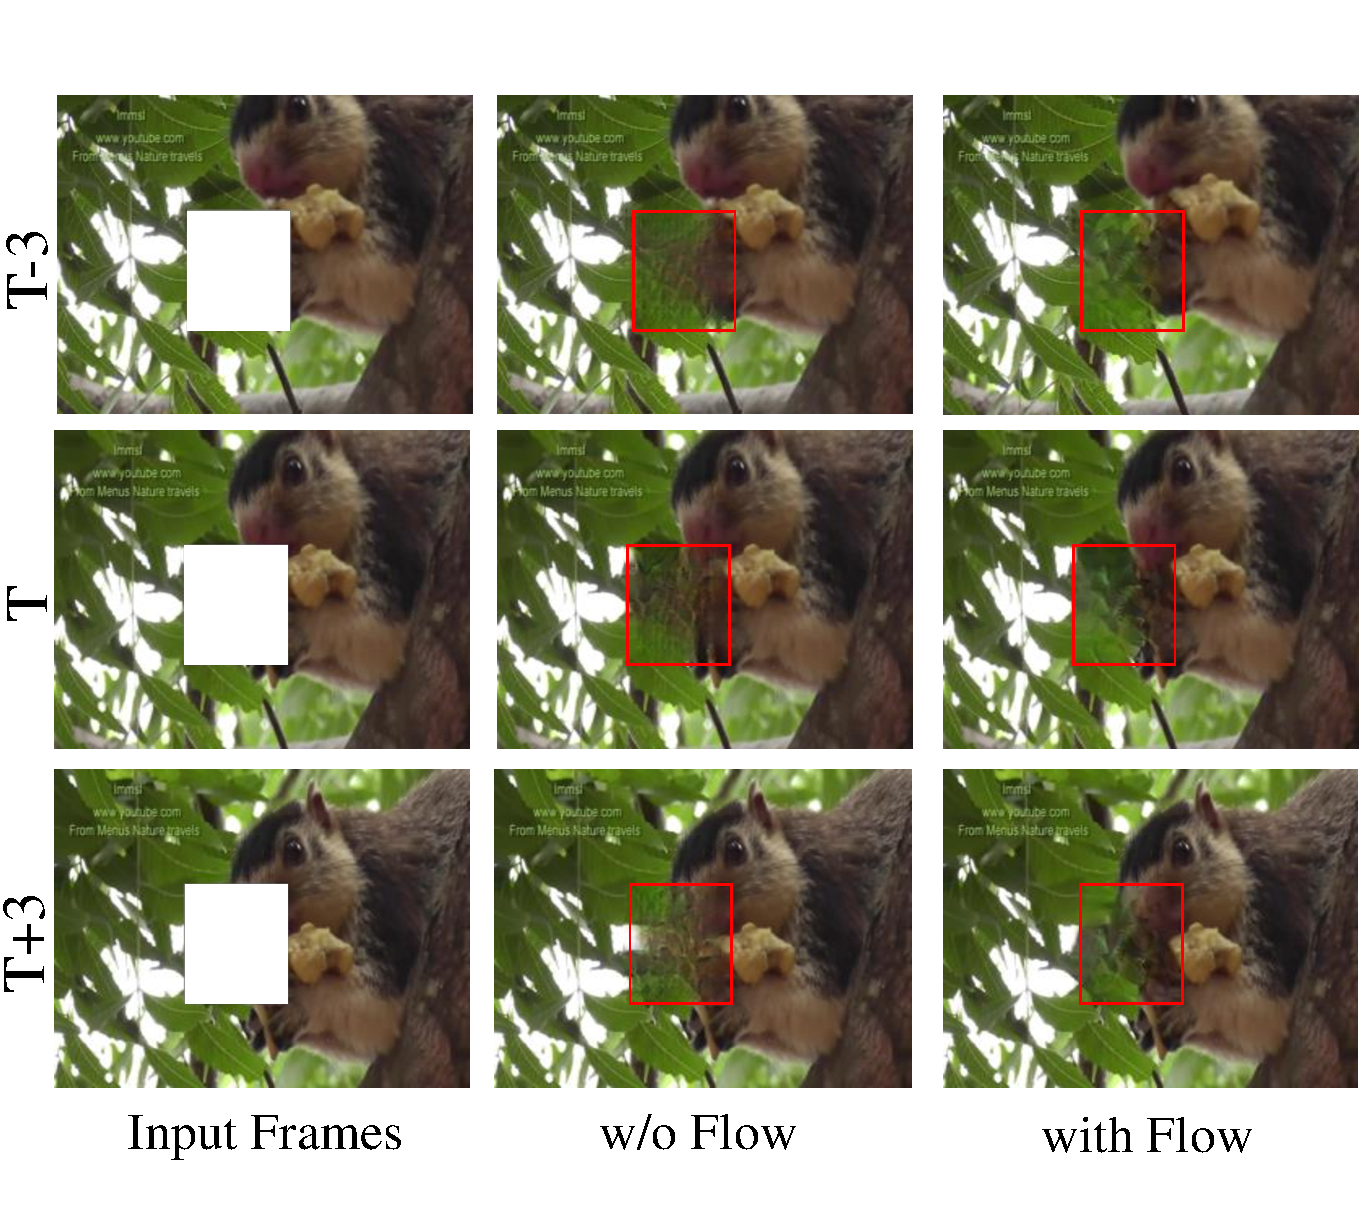
\includegraphics[width=0.9\columnwidth]{flow_vis} % Reduce the figure size so that it is slightly narrower than the column. Don't use precise values for figure width.This setup will avoid overfull boxes. 
	\caption{Inpainting results of three neighboring frames. With the flow constraints during network training, the inpainting results are more temporally consistent without introducing image blurs. }
	\label{flow_vis}
\end{figure}



\begin{figure}[t]
	\centering
	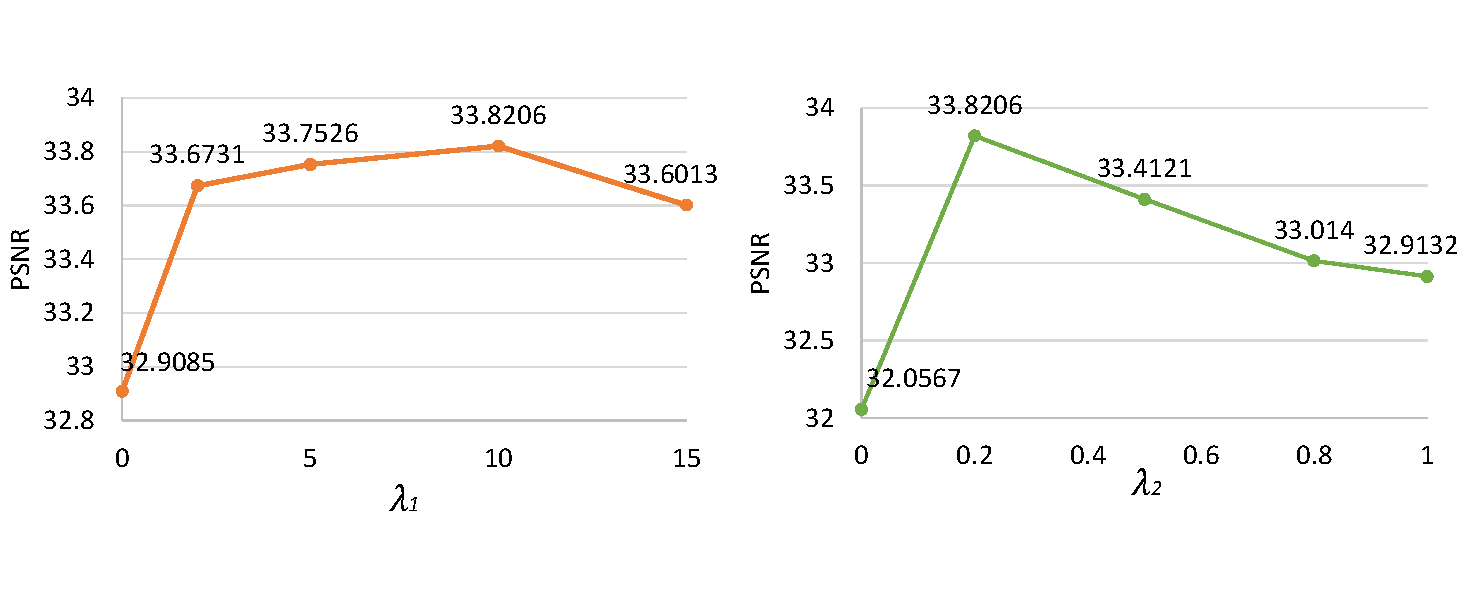
\includegraphics[width=1.0\columnwidth]{lamda1} % Reduce the figure size so that it is slightly narrower than the column. Don't use precise values for figure width.This setup will avoid overfull boxes. 
	\caption{Comparison of hyper parameters $\lambda_1$ and $\lambda_2$. The best result is obtained when $\lambda_1=10.0$ and $\lambda_2=0.2$.}
	\label{fig:hparam}
\end{figure}






 

